\section{Sufiksne strukture podataka}

\subsection{Sufiks niz}

Sufiks niz je struktura podataka koja omogu\' cava brzo tra\v zenje pojavljivanja stringa unutar stringa za koji se konstrui\v se sufiks niz, ta\v cnije, vremenska slo\v zenost pretrage je sublinearna funkcija du\v zine stringa unutar kojeg se vr\v si pretraga. Pored ovoga, pomo\' cu sufiks niza se mogu brzo vr\v siti pore\dj enja podstringova unutar samog stringa. \cite{sufiksnizprvirad}

Sufiks niz za string $s$ je niz sortiranih nepraznih sufiksa tog stringa. Formalno,

\begin{dfn}
Sufiks niz za string $s$ du\v zine $|s| = n$ je niz $p$ koji se sastoji od $n$ razli\v citih celih brojeva iz skupa $\{0,\ldots,n-1\}$ takav da je niz sufiksa \v cije su po\v cetne pozicije $p_0, p_1, \ldots, p_{n-1}$ leksikografski rastu\' ci niz.
\end{dfn}

Za svaki string postoji jedinstven sufiks niz, zato \v sto je leksikografsko ure\dj enje totalno a ne postoje dva jednaka sufiksa. Primera radi, na\dj imo sufiks niz za string \texttt{banana}. Ozna\v cimo sa $u_i$ string $s_{[i,n)}$. Svi sufiksi ovog stringa su:

\begin{center}
\begin{tabular}{cl}
    $u_0$ & \texttt{banana} \\
    $u_1$ & \texttt{anana} \\
    $u_2$ & \texttt{nana} \\
    $u_3$ & \texttt{ana} \\
    $u_4$ & \texttt{na} \\
    $u_5$ & \texttt{a} \\
\end{tabular}
\end{center}

Sortiranjem dobijamo niz sufiksa:

\begin{center}
\begin{tabular}{cl}
    $u_5$ & \texttt{a} \\
    $u_3$ & \texttt{ana} \\
    $u_1$ & \texttt{anana} \\
    $u_0$ & \texttt{banana} \\
    $u_4$ & \texttt{na} \\
    $u_2$ & \texttt{nana} \\
\end{tabular}
\end{center}

Sortirani niz sufiksa je $u_5, u_3, u_1, u_0, u_4, u_2$, pa je sufiks niz $p = (5,3,1,0,4,2)$.

\subsubsection{Konstrukcija}

Sufiks niz se mo\v ze konstruisati prostim sortiranjem svih sufiksa u vremenskoj slo\v zenosti $O(n^2 \log n)$, ukoliko je dostupan algoritam za sortiranje op\v ste namene koji radi u slo\v zenosti $O(n \log n)$. Primer takvog algoritam je \textit{mergesort}. Radi u\v stede memorijskog prostora sortira\' cemo samo niz celih brojeva $0,1,\ldots,n-1$, dok \' cemo kao funkciju za pore\dj enje koristiti funkciju koja je "svesna" stringa $s$ i koja za data dva sufiksa odre\dj uje koji je manji.

\noindent
\begin{minipage}[l]{\textwidth}
\lstinputlisting[language=C++, title={\textit{Implementacija klase za pore\dj enje sufiksa stringa}}, style=customcpp]{cpp/sarray-slow-cmp.h}
\end{minipage}

Vremenska slo\v zenost pore\dj enja dva sufiksa je $O(n)$, a kako \textit{mergesort} sortira niz sa $O(n \log n)$ poziva funkcije za pore\dj enje, ukupna vremenska slo\v zenost je $O(n^2 \log n)$.

\noindent
\begin{minipage}[l]{\textwidth}
\lstinputlisting[language=C++, title={\textit{Glavni algoritam za nala\v zenje sufiks niza, slo\v zenosti $O(n^2 \log n)$}}, style=customcpp]{cpp/sarray-slow.cpp}
\end{minipage}

\textit{Napomena.} Funkcija \texttt{iota} puni zadati opseg uzastopnim vrednostima po\v cev od tre\' ceg parametra, u ovom slu\v caju $0$. Koristimo je da niz $p$ inicijalizujemo vrednostima $p_i = i$. Prema standardu jezika, po\v cev od C++11, funkcija \texttt{sort} zove funkciju za pore\dj enje $O(n \log n)$ puta. \cite{sortnlogn} Tre\' ci parametar je funkcija ili drugi objekat koji ima implementiran \texttt{operator()} koji mo\v ze da poredi elemente niza.

Ozna\v cimo sa $k$ du\v zinu najdu\v zeg stringa koji se javlja vi\v se od jednom u stringu $s$. Nije te\v sko pokazati da, ako se pa\v zljivo implementira, funkcija pore\dj enja dva sufiksa radi u vremenskoj slo\v zenosti $O(k)$, pa se slo\v zenost konstrukcije sufiks niza mo\v ze i bolje proceniti sa $O(kn \log n)$.

\subsubsection{Br\v zi algoritmi za konstrukciju}

Algoritmi dati u nastavku efikasno re\v savaju problem nala\v zenja sortiranog niza svih cikli\v cnih pomeraja stringa. Prvo \' cemo pokazati kako se problem nala\v zenja sufiks niza svodi na sortiranje svih cikli\v cnih pomeraja stringa. Neka je $s \in \Sigma^+$. Pro\v sirimo alfabet $\Sigma$ dodavanjem novog simbola, koji \' cemo ozna\v citi sa $\$$ koji je po ure\dj enju manji od svih simbola iz $\Sigma$. Tada je $s' = s\$ \in (\Sigma \cup \{\$\})^+$. Neka je $n = |s|, n' = n+1 = |s'|$. Posmatrajmo sve cikli\v cne pomeraje stringa $s'$. Po\v sto se karakter $\$$ javlja samo jednom u stringu $s'$, svi ovi stringovi su razli\v citi pa postoji jedinstven leksikografski poredak. Leksikografski najmanji pomeraj bi\' ce $n'-1$, jer je taj pomeraj jedini koji po\v cinje karakterom $\$$ koji je po definiciji manji od svih ostalih.

\begin{thm}
Ako su $i,j$ proizvoljni cikli\v cni pomeraji stringa $s'$ razli\v citi od $n'-1$, tada va\v zi $s'_{[i, i+n')} < s'_{[j, j+n')}$ akko je $s_{[i, n)} < s_{[j, n)}$. \hfill $\square$
\end{thm}

Odavde sledi da ako je niz $q_0, q_1, \ldots, q_n$ sortiran niz cikli\v cnih pomeraja stringa $s'$ tada je niz $p_i = q_{i+1}, i \in \{0, \ldots, n-1\}$ sufiks niz stringa $s$.

\noindent
\begin{minipage}[l]{\textwidth}
\lstinputlisting[language=C++, title={\textit{Svo\dj enje konstrukcije sufiks niza na sortiranje cikli\v cnih pomeraja}}, style=customcpp]{cpp/scs-to-sarray.h}
\end{minipage}

Kona\v cno, opi\v simo algoritam za sortiranje cikli\v cnih pomeraja stringa $s$ du\v zine $n$. Za svako $k \in \{0, 1, \ldots, \ceil{\log_2(n)} \}$ na\dj imo poredak svih cikli\v cnih podstringova du\v zine $2^k$. Ovaj poredak \' cemo opisati nizom celih brojeva $C^{(k)}$, gde stringu $s_{[i, i+2^k)}$ pridru\v zujemo broj $C^{(k)}_i$ na takav na\v cin da, ako su podstringovima $s_{[i, i+2^k)}$ i $s_{[j, j+2^k)}$ pridru\v zeni isti brojevi, tada su oni jednaki, a ako je jednom pridru\v zen manji broj, tada je taj podstring leksikografski manji. Za $k=0$, mo\v zemo jednostavno postaviti $C^{(0)}_i = \text{Ord}(s_i)$.

Neka je $k>0$. Na\v s cilj je da odredimo niz $C^{(k)}$ u vremenskoj slo\v zenosti $O(n \log n)$. Posmatrajmo podstringove $s_{[i, i+2^k)}$ i $s_{[j, j+2^k)}$ i posmatrajmo ure\dj ene parove $u_i = (C^{(k-1)}_i, C^{(k-1)}_{(i+2^{k-1}) \mod n })$ i $u_j = (C^{(k-1)}_j, C^{(k-1)}_{(j+2^{k-1}) \mod n })$. Tada je poredak ovih podstringova jednak poretku parova $u_i, u_j$. Ako za svaki cikli\v cni podstring odredimo ovaj ure\dj eni par, zatim sve dobijene parove sortiramo, a zatim ovim parovima dodelimo ordinalne vrednosti, dobi\' cemo upravo niz $C^{(k)}$. Ovo se mo\v ze jednostavno izvesti bilo kojim algoritmom za sortiranje koji radi u slo\v zenosti $O(n \log n)$.

Za kraj, neka je $k = \ceil{\log_2(n)}$. Odavde je $2^k \geq n$. U kontekstu konstrukcije sufiks niza, nijedna dva cikli\v cna pomeraja du\v zine $2^k$ ne\' ce biti jednaka, pa \' ce niz $C^{(k)}$ sadr\v zati razli\v cite brojeve. Odavde sortiran niz cikli\v cnih pomeraja mo\v zemo na\' ci kao inverznu permutaciju niza $C^{(k)}$. Va\v zno je napomenuti da \' ce poredak podstringova du\v zine $2^k$ biti jednak poretku podstringova du\v zine $n$, zato \v sto du\v zina najdu\v zeg zajedni\v ckog prefiksa za bilo koja dva razli\v cita podstringa (bilo koje du\v zine) iznosi $n-1$, upravo jer postoji karakter $\$$ koji se javlja samo jednom u stringu.

Kako ovaj algoritam ima $O(\log n)$ faza, a svaka faza radi u slo\v zenosti $O(n \log n)$, ukupna vremenska slo\v zenost je $O(n \log^2 n)$. Memorijska slo\v zenost je $O(n \log n)$, ali se mo\v ze smanjiti na $O(n)$ pam\' cenjem samo nizova $C^{(k)}$ prethodne i trenutne faze.

\noindent
\begin{minipage}[l]{\textwidth}
\lstinputlisting[language=C++, title={\textit{Algoritam za sortiranje cikli\v cnih pomeraja, slo\v zenosti $O(n \log^2(n))$}}, style=customcpp]{cpp/sarray-medium.cpp}
\end{minipage}

Prethodno opisani algoritam za nala\v zenje cikli\v cnih pomeraja je mogu\' ce modifikovati tako da radi u slo\v zenosti $O(n \log n)$. Naime, ukoliko bismo sortirali parove $u_i$ u linearnom vremenu, dobili bismo upravo tu vremensku slo\v zenost. Svaki par se sastoji iz dva broja iz skupa $\{0, 1, \ldots, n-1\}$. Mo\v zemo primeniti ideju iz algoritma \textit{radix sort}. Naime, \textit{radix sort} se oslanja na \textit{counting sort}, koji ima jednostavnu implementaciju i mo\v ze da sortira bilo koji niz od $n$ elemenata \v ciji su klju\v cevi za pore\dj enje brojevi iz skupa $\{0, 1, \ldots, k-1\}$ u vremenskoj slo\v zenosti $O(n+k)$. Pritom, mogu\' ce je implementirati \textit{counting sort} kao stabilan algoritam sortiranja, odnosno algoritam koji ekvivalentnim elementima ne menja relativni poredak. Algoritam \textit{radix sort} za ure\dj ene parove bi prvo pomo\' cu \textit{counting sort}-a sortirao sve parove po drugom elementu, a zatim po prvim, vode\' ci ra\v cuna da se ne naru\v si prethodno ustanovljen poredak kori\v s\' cenjem stabilne varijante \textit{counting sort}-a.

Mogu\' ce je pojednostaviti prethodni algoritam, odnosno, svesti ga na samo jedno pozivanje \textit{counting sort}-a. Naime, pored nizova $C^{(k)}$ \v cuva\' cemo eksplicitno i permutaciju $p^{(k)}$ koja odgovara poretku podstringova du\v zine $2^k$. Posmatrajmo \v sta se de\v sava ukoliko pomo\' cu \textit{counting sort}-a sortiramo vrednosti $(j - 2^{k-1}) \mod n$, gde je klju\v c $C^{(k-1)}_{(j - 2^{k-1}) \mod n}$, uzete redom za svako $j$ iz niza $p^{(k-1)}$. Stabilan \textit{counting sort} \' ce urediti ove indekse $j' = (j - 2^{k-1}) \mod n$ po vrednosti $C^{(k-1)}_{j'}$, dok \' ce, ukoliko vi\v se njih ima istu vrednost, o\v cuvati prethodno ustanovljeni poredak. Kako je ovaj prethodni poredak indukovan vrednostima $C^{(k-1)}_j = C^{(k-1)}_{(j' + 2^{k-1}) \mod n}$, dobijamo upravo leksikografski redosled parova $(C^{(k-1)}_{j'}, C^{(k-1)}_{(j' + 2^{k-1}) \mod n})$. Sada na osnovu ovog sortiranog niz ra\v cunamo nove vrednosti $C^{(k)}$, dok je $p^{(k)}$ dobijen upravo pomenutim sortiranjem.

Kona\v cno re\v senje, odnosno sortiran niz cikli\v cnih pomeraja je upravo niz $p^{(k)}$ za $k = \ceil{\log_2(n)}$.

\noindent
\begin{minipage}[l]{\textwidth}
\lstinputlisting[language=C++, title={\textit{Algoritam za sortiranje cikli\v cnih pomeraja, slo\v zenosti $O(n \log n)$}}, style=customcpp]{cpp/sarray-fast.cpp}
\end{minipage}

\subsubsection{LCP niz}

Niz najdu\v zih zajedni\v ckih prefiksa (\textit{longest common prefix}) je niz koji se \v cesto zajedno koristi sa sufiks nizom. Za string $s$ du\v zine $n$, \v ciji je sufiks niz $p_0, p_1, \ldots, p_{n-1}$, LCP niz se sastoji od nenegativnih celih brojeva $q_0, q_1, \ldots, q_{n-2}$, gde $q_i$ ozna\v cava du\v zinu najdu\v zeg zajedni\v ckog prefiksa stringova $s_{[p_i, n)}$ i $s_{[p_{i+1}, n)}$.

Najdu\v zi zajedi\v cki prefiks zadovoljava jednu veoma va\v znu osobinu.

\begin{thm}
\label{lcposobina}
Neka je $s_1, s_2, s_n$ leksikografski sortiran niz stringova. Neka je $q_i = LCP(s_i, s_{i+1})$. Ako je $i<j$, tada je $LCP(s_i, s_j) = \min\{q_i, q_{i+1}, \ldots, q_{j-1}\}$. \hfill $\square$
\end{thm}

Kako se LCP niz konstrui\v se nad sortiranim nizom sufiksa jednog stringa, on se uz odgovaraju\' cu strukturu podataka za nala\v zenje minimuma u podnizu mo\v ze koristiti za odre\dj ivanje najdu\v zeg zajedni\v ckog prefiksa bilo koja dva sufiksa.

Pre nego \v sto opi\v semo algoritam za konstrukciju LCP niza, doka\v zimo slede\' cu teoremu.

\begin{thm}
\label{lcpalgoteorema}
Neka je $s$ string du\v zine $n$, \v ciji je sufiks niz $p_0, \ldots, p_{n-1}$, LCP niz $q_0, \ldots, q_{n-2}$. Defini\v semo $r = p^{-1}$ odnosno, $p_{r_i} = i$. Neka je $s_{[i, n)}$ njegov sufiks takav da je $i>0$ i $p_{n-1} \not = i, i-1$. Tada je $q_{r_i} \geq q_{r_{i-1}} - 1$.
\end{thm}

\textit{Dokaz:} Uvedimo oznake $i' = i-1$, $j = p_{r_i + 1}$, $j' = p_{r_{i'} + 1}$. Drugim re\v cima, sufiks $i'$ je onaj koji prethodi $i$, odnosno ima du\v zinu za $1$ ve\' cu. $j$ je sufiks koji se nalazi odmah posle $i$ u sufiks nizu. Sli\v cno, $j'$ je sufiks koji se nalazi odmah posle $i'$ u sufiks nizu.  Ukoliko je $q_{r_{i'}} \leq 1$, onda tvr\dj enje o\v cigledno va\v zi, jer je $q_{r_i} \geq 0$. Neka je $q_{r_{i'}} \geq 2$. Po\v sto je $j'$ posle $i'$ u sufiks nizu va\v zi $s_{[j', n)} > s_{[i', n)}$ a po\v sto je $q_{r_{i'}} \geq 1$ va\v zi $s_{i'} = s_{j'}$. Ako odbacimo prvi karakter sufiksa $i'$ i $j'$ ponovo dobijamo sufikse, $i'+1, j'+1$ i va\v zi $s_{[j'+1, n)} > s_{[i'+1, n)}$, odnosno $s_{[j'+1, n)} > s_{[i, n)}$ ili ekvivalentno $r_{j'+1} > r_i$. Du\v zina najdu\v zeg zajedni\v ckog prefiksa za $i'+1, j'+1$ je $q_{r_{i'}} - 1$. Na osnovu teoreme \ref{lcposobina} imamo da je $q_{r_{i'}} - 1 = LCP(s_{[i, n)}, s_{[j'+1, n)}) = \min\{ q_{r_i}, q_{r_i+1}, \ldots, q_{r_{j'+1}-1} \}$ odnosno $q_{r_{i'}} - 1 \leq q_{r_i}$ \hfill $\square$.

Algoritam za konstrukciju LCP niza\cite{lcpnizrad} radi na slede\' ci na\v cin. Kao ulaz se prosle\dj uju string i izra\v cunati sufiks niz tog stringa. Prvo se ra\v cuna inverz sufiksnog niza. Zatim se sufiksi obra\dj uju redom, opadaju\' ce po du\v zini, odnosno, uzimaju se redom sufiksi \v cije su po\v cetne pozicije $i = 0, 1, \ldots, n-1$ tim redom. U svakom trenutku odr\v zavamo promenljivu $k$ koja je manja ili jednaka od trenutne vrednosti $q_{r_i}$ koju tra\v zimo. U po\v cetku je $k=0$. Ukoliko je $r_i = n-1$, $q_{r_i}$ se i ne defini\v se i samo postavljamo $k=0$. U suprotnom, samo pove\' cavamo $k$ za po $1$ sve dok se odgovaraju\' ci karakteri sufiksa $i$ i $j = p_{r_i + 1}$ poklapaju. Kada do\dj emo do kraja nekog od ovih sufiksa ili se karakteri ne poklope, prekidamo, upisujemo $q_{r_i} := k$ i zatim, na osnovu teoreme \ref{lcpalgoteorema} smemo da postavimo $k := \max\{k-1, 0\}$.

\noindent
\begin{minipage}[l]{\textwidth}
\lstinputlisting[language=C++, title={\textit{Algoritam za nala\v zenje LCP niza}}, style=customcpp]{cpp/lcp-array.cpp}
\end{minipage}

Vremenska slo\v zenost ovog algoritma je $O(n)$ za ra\v cunanje inverza i petlju koja redom obra\dj uje sufikse, plus linearna po ukupnom broju uve\' cavanja promenljive $k$. Kako u ta\v cno jednoj iteraciji (kad je $r_i = n-1$) $k$ smanjujemo direktno na $0$, a u svim ostalim iteracijama $k$ smanjujemo za najvi\v se $1$, ukupno je smanjujemo za najvi\v se $2n-2$. Kako je po\v cetna vrednost $0$ a krajnja ne vi\v se od $n-1$, to zna\v ci da je $k$ pove\' cavamo najvi\v se $3n-3$, odnosno $O(n)$ puta, pa ceo algoritam radi u slo\v zenosti $O(n)$.

\subsubsection{Primene}

\noindent
\textbf{Tra\v zenje jednog stringa u drugom}

Ukoliko je potrebno tra\v ziti veliki broj stringova, recimo njih $m$ unutar jednog istog stringa $s$ du\v zine $n$, pritom, za svaki od tih stringova je neophodno odmah na\' ci odgovor pre nego \v sto se po\v cne sa obradom slede\' ceg, bez preprocesiranja stringa $s$ bi\' ce nam potrebno bar $O(nm)$ vremena. Ukoliko su stringovi koji se tra\v ze mnogo manje du\v zine od $n$, recimo, svaki je du\v zine $d$, onda bi algoritam slo\v zenosti $O(md\log n)$ radio mnogo br\v ze.

Pomo\' cu sufiks niza realizacija algoritma koji tra\v zi string $t$ du\v zine $d$ u stringu $s$ je krajnje jednostavna. Binarnom pretragom po sufiks nizu tra\v zimo prvu poziciju takvu da je odgovaraju\' ci sufiks leksikografski ve\' ci ili jednak tra\v zenom stringu. Kako se pore\dj enje bilo kog sufiksa i stringa $p$ mo\v ze izvr\v siti u vremenu $O(d)$, slo\v zenost pretrage je $O(d \log n)$.

Slede\' ca implementacija nalazi \textit{lower bound} za string $t$, odnosno, najmanji broj $i$ takav da je $s_{[p_i, n)} \leq t$, ili $i=n$ ukoliko takav broj ne postoji.

\noindent
\begin{minipage}[l]{\textwidth}
\lstinputlisting[language=C++, title={\textit{Tra\v zenje lower bound-a pomo\' cu sufiks niza}}, style=customcpp]{cpp/sarray-lb.cpp}
\end{minipage}

Prethodni algoritam se mo\v ze iskoristiti za tra\v zenje pojavljivanja stringa $t$ u stringu $s$, tako \v sto za na\dj eni broj $i$ uporedimo stringove $s_{[p_i, p_i + d))}$ i $t$, naravno, ukoliko je $p_i + d \leq n$.

\noindent
\begin{minipage}[l]{\textwidth}
\lstinputlisting[language=C++, title={\textit{Tra\v zenje podstringa pomo\' cu sufiks niza}}, style=customcpp]{cpp/sarray-find.cpp}
\end{minipage}

\noindent
\textbf{Leksikografski najmanji cikli\v cni pomeraj}

Pomo\' cu algoritma za sortiranje cikli\v cnih pomeraja mo\v zemo lako utvrditi koji cikli\v cni pomeraj je najmanji, tako \v sto direktno primenimo tu funkciju na string bez dodavanja novog, minimalnog karaktera. \v Stavi\v se, jednostavno mo\v zemo na\' ci i minimalnu periodu stringa $s$ du\v zine $n$, odnosno, najmanji prirodan broj $l$ takav da je $s_i = s_{(i+l) \mod n}$ za svako $i$. To je upravo broj razli\v citih elemenata niza $C^{(k)}$ za $k = \ceil{\log_2(n)}$.

\noindent
\textbf{Leksikografsko pore\dj enje podstringova}

Ukoliko kod algoritma za sortiranje cikli\v cnih pomeraja upamtimo sve nizove $C^{(k)}$, mo\v zemo vrlo jednostavno vr\v siti leksikografsko pore\dj enje podstringova, uklju\v cuju\' ci i cikli\v cne podstringove. Ukoliko treba da uporedimo dva stringa razli\v citih du\v zina, recimo $l_1 < l_2$, prvo uporedimo kra\' ci od njih sa prefiksom du\v zeg du\v zine $l_1$. Ukoliko dobijemo da su ti stringovi razli\v citi, prekidamo, ina\v ce, po definiciji, leksikografski manji string je kra\' ci. Zato pretpostavimo da upore\dj ujemo podstringove iste du\v zine, neka su to $s_{[i, i+l)}, s_{[j, j+l)}$.  Ukoliko je $l = 2^k$ za neko $k$, mo\v zemo prosto uporediti vrednosti $C^{(k)}_i$ i $C^{(k)}_j$. U suprotnom, na\dj imo najve\' ce $k$ takvo da je $2^k < l$. Pritom, jasno je da va\v zi $2^k > \frac{l}{2}$. Ideja je da prvo uporedimo prefikse ovih stringova du\v zine $2^k$ isto kao u prethodnom slu\v caju. Ukoliko dobijemo da su prefiksi jednaki, uporedimo njihove sufikse du\v zine $2^k$ -- rezultat ovog pore\dj enja bi\' ce rezultat pore\dj enja celih stringova.

Jasno je da ovaj algoritam radi u slo\v zenosti $O(1)$ ali zato koristi $O(n \log n)$ memorije za nizove $C^{(k)}$. Mogu\' ce je dosti\' ci istu vremensku slo\v zenost za pore\dj enje sa samo $O(n)$ dodatne memorije kori\v s\' cenjem LCP niza. Ideja je da, pri pore\dj enju podstringova $s_{[i, i+l)}, s_{[j, j+l)}$ na\dj emo $d = LCP(s_{[i, n)}, s_{[j, n)})$, Ukoliko je $d < l$, samo uporedimo karaktere $s_{i+d}, s_{j+d}$, ina\v ce, stringovi su jednaki. Na osnovu teoreme \ref{lcposobina} problem se svodi na nala\v zenje minimuma u podsegmentu niza. Ovaj problem se mo\v ze efikasno re\v siti u vremenskoj slo\v zenosti $O(1)$ sa $O(n)$ preprocesiranja i $O(n)$ utro\v sene memorije \cite{lcarmqrad}.

\subsection{Sufiks stablo}

Sufiks stablo je struktura podataka koja uop\v stava sufiks niz i usko je povezana sa njim. Da bismo definisali sufiksno stablo, defini\v simo prvo kompresovano prefiksno stablo.

\begin{dfn}
Kompresovano prefiksno stablo za skup nepraznih stringova $P$ se dobija tako \v sto se u prefiksnom stablu obri\v su svi \v cvorovi vi\v sestrukosti $0$ sa ta\v cno jednim detetom, osim korena, a zatim se dodaju grane koje odgovaraju obrisanim putevima u stablu i imaju labele koje odgovaraju obrisanim putevima.
\end{dfn}

\begin{figure}[H]
    \centering
    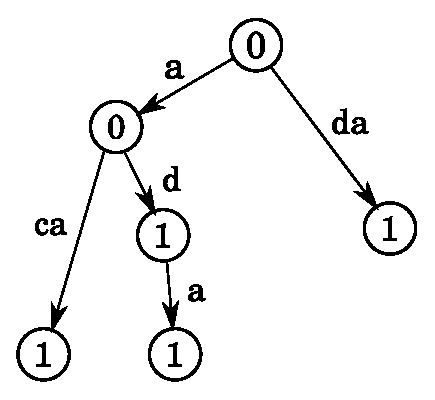
\includegraphics[width=75mm]{../img/ztrie1.eps}
    \caption*{\textit{Kompresovano prefiksno stablo za skup $\{aca,ad,ada,da\}$.}}
\end{figure}

U primeru sa slike, \v cvor $\delta(ad)$ ne bri\v semo iako on ima jedno dete. Najzad, defini\v simo sufiks stablo.

\begin{dfn}
Sufiks stablo za string $s$ je kompresovano prefiksno stablo svih nepraznih sufiksa stringa $s$.
\end{dfn}

Iako na prvi pogled deluje da bi ovakvo stablo zauzimalo previ\v se memorije i iz tog razloga bilo neprakti\v cno, pokazuje se suprotno.

\begin{thm}
Kompresovano prefiksno stablo od $n$ stringova sadr\v zi najvi\v se $2n$ \v cvorova. 
\end{thm}

\textit{Dokaz.} Indukcijom po $n$. Za $n=1$ tvr\dj enje o\v cigledno va\v zi. Posmatrajmo stablo za skup stringova $P' = P - p$. Neka je $q$ najdu\v zi prefiks stringa $p$ koji se javlja u $P'$. Ukoliko ne postoji \v cvor $\delta(q)$, put od korena sa labelom $q$ \' ce odgovarati unutra\v snjosti neke grane, pa ovu granu delimo na dve umetanjem novog \v cvora koji \' ce onda biti $\delta(q)$. Zatim, ukoliko je $|q| < |p|$ dodajemo novu granu iz \v cvora $\delta(q)$ ka novom \v cvoru i upisujemo joj labelu $p_{[|q|, |p|)}$. Broj \v cvorova se pove\' cao za najvi\v se $2$, \v sto dokazuje tvr\dj enje. \hfill $\square$

Naizgled, \v cak iako stablo ima mali broj \v cvorova, ukupna du\v zina labela svih grana mo\v ze biti $\Theta(n^2)$, \v sto bi impliciralo veliku memorijsku slo\v zenost. Kod sufiks stabla, sve labele grana su podstringovi stringa $s$ pa umesto stringa labelu mo\v zemo predstaviti kao par $l,r$ koji bi ozna\v cavao da je labela te grane jednaka stringu $s_{[l, r)}$.

Postoje algoritmi koji konstrui\v su sufiks stablo direktno iz datog stringa u linearnom vremenu \cite{suffixtreerad}. U nastavku \' ce biti prezentovan jednostavan algoritam koji na osnovu izra\v cunatih sufiks i LCP nizova konstrui\v se sufiks stablo.

\noindent
\begin{minipage}[l]{\textwidth}
\lstinputlisting[language=C++, title={\textit{Struktura \v cvora sufiks stabla}}, style=customcpp]{cpp/stree_node.h}
\end{minipage}

Svaki \v cvor sufiks stabla pamti labelu grane koja spaja taj \v cvor i njegovog roditelja, odnosno podstring stringa $s$, pokaziva\v c na svog roditelja kao i pokaziva\v ce na svoju decu. Umesto vi\v sestrukosti pamti se redni broj $id$ takav da je taj \v cvor jednak $\delta(s_{[id,n)})$ ukoliko postoji, ina\v ce $-1$, \v sto odgovara \v cvorovima vi\v sestrukosti $0$. Za koren stabla se ne defini\v se roditelj a brojeve $l,r$ postavljamo na $0$. Iz definicije sufiks stabla zaklju\v cujemo da sve grane koji izlaze iz jednog \v cvora imaju labele kojima se razlikuje prvo slovo, \v sto opravdava izbor mape za \v cuvanje izlaznih grana. Algoritam radi na slede\' ci na\v cin. U leksikografskom redosledu se dodaju sufiksi stringa $s$. Ovaj redosled je odre\dj en sufiks nizom $p$. Prvi string se dodaje kao zasebna grana. Za svaki naredni string, odnosno $i$-ti za $i>0$, va\v zi da je najdu\v zi zajedni\v cki prefiks njega i bilo kog drugog stringa upravo jednak $q_{i-1}$ (Teorema \ref{lcposobina}). Penjemo se od kraja prethodno uba\v cenog sufiksa do dubine $q_{i-1}$ u stablu, mereno po broju slova u labelama. Ukoliko se pozicija na ovoj visini nalazi na sredini grane, delimo tu granu na dva dela. Kona\v cno, ostaje nam da dodamo deo zavr\v sni deo sufiksa du\v zine $(n-p_i)-q_{i-1}$, naravno, samo ako je on neprazan.

\noindent
\begin{minipage}[l]{\textwidth}
\lstinputlisting[language=C++, title={\textit{Implementacija algoritma za konstrukciju sufiks stabla}}, style=customcpp]{cpp/suffix-tree.cpp}
\end{minipage}

Vremenska slo\v zenost ovog algoritma je $O(n)$. Ovo se mo\v ze dokazati tako \v sto posmatramo vrednost $2i-y$, gde je $y$ dubina \v cvora $curr$ u stablu, merena po broju grana. Svaka iteracija i spoljne \textit{for} i unutra\v snje \textit{while} petlje uve\' cava vrednost ovog izraza za bar $1$, pa je njihov ukupan broj manji od $2n$.

Sufiks stablo omogu\' cava da se na\dj u prvo, poslednje, broj pojavljivanja nekog stringa $t$ unutar stringa $s$ u linearnom vremenu procedurom spu\v stanja sli\v cno kao kod prefiksnog stabla. Kod tra\v zenja svih pojavljivanja stringa korisna je slede\' ca teorema:

\begin{thm}
Kod sufiksnog stabla ne postoji podstablo koje sadr\v zi vi\v se \v cvorova vi\v sestrukosti $0$ nego \v cvorova vi\v sestrukosti $1$.
\end{thm}

\textit{Dokaz.} Pretpostavimo suprotno, da podstablo ima $k$ \v cvorova i da \v cvorova vi\v sestrukosti $0$ ima vi\v se od $\frac{k}{2}$. Na osnovu definicije sufiks stabla, svaki takav \v cvor ima bar dvoje dece, pa je ukupan broj dece svih \v cvorova u podstablu ve\' ci od $k$, \v sto je nemogu\' ce, jer je ukupan broj dece svih \v cvorova ta\v cno $k-1$.

Ovo nam omogu\' cava da, za neki string $t$, od pozicije $\delta(t)$, ukoliko postoji, izvr\v simo pretragu u dubinu ili \v sirinu da bismo na\v sli sve \v cvorove vi\v sestrukosti $1$ u podstablu pozicije $\delta(t)$. Ako neki ovakav \v cvor odgovara sufiksu $id$, znamo da je $t = s_{[id, id+|t|)}$ odnosno, $id$ je pozicija jednog pojavljivanja stringa $t$ u stringu $s$. Kako je slo\v zenost pretrage linearna po veli\v cini podstabla, i kako je ukupan broj \v cvorova podstabla ne vi\v se od duplo ve\' ci od broja \v cvorova vi\v sestrukosti $1$, vremenska slo\v zenost algoritma je $O(|t|+k)$, gde je $k$ broj pojavljivanja stringa $t$ u $s$.

Od konstruisanog sufiks stabla se mo\v ze dobiti sufiks niz tra\v zenjem praznog stringa, ili ekvivalentno, pu\v stanjem pretrage u dubinu od korena i pam\' cenjem $id$ vrednosti za sve \v cvorove za koje je $id \not = -1$.

\noindent
\begin{minipage}[l]{\textwidth}
\lstinputlisting[language=C++, title={\textit{Nala\v zenje svih pojavljivanja stringa $t$ u stringu $s$}}, style=customcpp]{cpp/stree-findall.cpp}
\end{minipage}

\textit{Napomena.} Prikazani kod ne vra\' ca sve pozicije u rastu\' cem, ve\' c u proizvoljnom redosledu.

\subsection{Sufiks automat}

\subsubsection{Definicija}

Sufiks automat je struktura podataka koja se gradi od datog stringa, a iz koje se mogu izvu\' ci razli\v cite korisne informacije o samom stringu i mo\v ze se koristiti za brzu pretragu podstringova, sli\v cno sufiks nizu i sufiks stablu. Glavna prednost sufiks automata je ta \v sto ima veoma jednostavan algoritam za konstrukciju koji radi u linearnom vremenu.

\begin{dfn}
Sufiks automat je parcijalni kona\v cni automat sa minimalnim brojem \v cvorova koji prepoznaje sve sufikse stringa $s$.
\end{dfn}

Parcijalni kona\v cni automat koji raspoznaje skup stringova $S \subseteq \Sigma^*$ je usmeren graf $(V,E)$, gde svaka grana ima labelu koja je slovo iz alfabeta $\Sigma$, zajedno sa specijalnim \v cvorom $t_0 \in V$, i skupom \v cvorova $T \subseteq V$, takav da je $s \in S$ akko postoji put od \v cvora $v_0$ do nekog \v cvora $t \in T$ \v ciji je niz labela $s$, i nijedan \v cvor nema dve izlazne grane sa istom labelom.

Pri odre\dj ivanju oblika sufiks automata, od velike koristi je $endpos$ funkcija. Ispostavi\' ce se da upravo ova funkcija odre\dj uje stanja, odnosno \v cvorove automata. Na dalje, smatrajmo da je $s$ fiksiran string du\v zine $n$ za koji konstrui\v semo sufiks automat.

\begin{dfn}
Za string $p$, $endpos(p)$ je skup celih brojeva takav da je $i \in endpos(p)$ akko je $|p| \leq i \leq |s|$ i $s_{[i-|p|,i)} = p$.
\end{dfn}

Drugim re\v cima, $endpos(p)$ je skup svih pojavljivanja stringa $p$ u $s$, gde za poziciju uzimamo desni kraj.

\begin{dfn}
Za stringove $p_1,p_2$, koji su podstringovi stringa $s$ ka\v zemo da su \textit{endpos}-ekvivalentni ukoliko va\v zi $endpos(p_1) = endpos(p_2)$.
\end{dfn}

Ukoliko su $p_1,p_2$ \textit{endpos}-ekvivalentni, tada je jedan od njih sufiks drugog. Svaka klasa ekvivalencije se sastoji od nekoliko stringova koji se mogu pore\dj ati u niz takav da je svaki naredni string sufiks prethodnog i ima du\v zinu za jedan manju. Samim tim, za predstavnika klase mo\v zemo uzeti najdu\v zi string te klase. Obrat ovog tvr\dj enja ne va\v zi, ali va\v zi da ako je $p_1$ sufiks stringa $p_2$, da je $endpos(p_2) \subseteq endpos(p_1)$. Tako\dj e, ako $p_1$ nije sufiks od $p_2$ i $p_2$ nije sufiks od $p_1$, tada je $endpos(p_1) \cap endpos(p_2) = \emptyset$. \cite{suffixautomatonrad}

Sufiks automat kao \v cvorove ima sve klase \textit{endpos}-ekvivalencije takve da je njima pridru\v zen \textit{endpos} skup neprazan. Sve izlazne grane nekog \v cvora se odre\dj uju na slede\' ci na\v cin. Neka je $u$ \v cvor automata odnosno jedna klasa ekvivalencije i neka je $p$ bilo koji string klase $u$. Za svako $x \in \Sigma$, ako je $px$ podstring od $s$, onda postoji grana od $u$ do klase koja sadr\v zi $px$. Primetimo da rezultat ne zavisi od izbora stringa $p$ iz klase $u$. Zaista, $endpos(px)$ je skup svih brojeva $i+1$ takvih da je $s_i = x, i \in endpos(p)$, pa grana ide ka klasi koja odgovara vrednosti $endpos(px)$. Ako posmatramo najkra\' ci string klase ekvivalencije $u$, osim klase koja sadr\v zi prazan string, uklanjanjem prvog slova tog stringa dobijamo druga\v ciju klasu ekvivalencije $v$, odnosno klasu koja sadr\v zi prethodni $endpos$ skup kao svoj strogi podskup. Ka\v zemo da postoji sufiks veza od \v cvora $u$ do \v cvora $v$ u automatu. Svi \v cvorovi imaju jedinstvenu izlaznu sufiks vezu, osim \v cvora koji odgovara praznom stringu, i veza uvek ide ka klasama koje sadr\v ze kra\' ce stringove, pa je dobijeni graf sufiks veza stablo.

\subsubsection{Algoritam za konstrukciju}

Opi\v simo algoritam koji konstrui\v se sufiks automat. Pored prethodno opisanih izlaznih grana, svaki \v cvor grafa \' ce pamtiti i du\v zinu najdu\v zeg stringa svoje klase ekvivalencije, kao i sufiks vezu.

\noindent
\begin{minipage}[l]{\textwidth}
\lstinputlisting[language=C++, title={\textit{Struktura \v cvora sufiks automata}}, style=customcpp]{cpp/sautomaton-node.h}
\end{minipage}

Algoritam radi u iteracijama, dodaju\' ci jedno po jedno slovo stringa $s$. Nakon $k$-te iteracije dobijeni graf odgovara sufiks automatu za string $s_{[0, k)}$. Algoritam po\v cinje inicijalizacijom po\v cetnog \v cvora koji odgovara klasi koja sadr\v zi prazan podstring. Dakle, $len$ se postavlja na $0$, $link$ na \textit{null}-pokaziva\v c, a skup prelaza je prazan. Tako\dj e, u svakom trenutku pamtimo i pokaziva\v c na \v cvor koji odgovara klasi koja sadr\v zi ceo string do tog trenutka, to je \v cvor $last$.

Posmatrajmo promene koje se dese na grafu nakon dodavanja karaktera $s_k$. Sigurno \' ce se javiti nova klasa koja \' ce sadr\v zati ceo string $s_{[0, k+1)}$ i mo\v zda jo\v s neke njegove sufikse. Ta\v cnije, ta klasa \' ce sadr\v zati sve sufikse stringa $s_{[0, k+1)}$ koji se ne javljaju ve\' c u stringu $s_{[0, k)}$. Taj novi \v cvor nazovimo $curr$. Njegova du\v zina je $k+1$, odnosno za jedan ve\' ca nego kod \v cvora $last$. Koji sve \v cvorovi imaju grane koje idu ka \v cvoru $curr$? To su neki od \v cvorova koji odgovaraju stanjima koja sadr\v ze sufikse stringa $s_{[0,k)}$. Podelimo sve ove sufikse u dve grupe, na one koji se javljaju u stringu $s_{[0,k)}$ na takav na\v cin da se neko od tih pojavljivanja mo\v ze produ\v ziti slovom $s_k$ unutar $s_{[0,k)}$, i one kod kojih to ne va\v zi. Jasno je da \' ce na ovaj na\v cin ovi sufiksi biti podeljeni po du\v zini u odnosu na neku granicu. Svim stanjima koja odgovaraju du\v zim sufiksima treba dodati granu sa labelom $s_k$ ka \v cvoru $curr$, dok kra\' ci sufiksi ve\' c imaju takvu granu, i te grane pokazuju na ve\' c postoje\' ce \v cvorove, pa ne treba raditi ni\v sta. Sve ove \v cvorove mo\v zemo obi\' ci tako \v sto krenemo od \v cvora $last$ i kre\' cemo se du\v z sufiks veza.

Neka je $p$ \v cvor na kojem smo se zaustavili. Podsetimo se da sufiks veza iz nekog \v cvora ide ka \v cvoru koji sadr\v zi najdu\v zi sufiks stringa tog \v cvora koji se javlja na vi\v se mesta od njega samog. Za \v cvor $curr$ potrebno je na\' ci string koji je sufiks stringa $s_{[0,k+1)}$ a javlja se jo\v s negde u stringu $s_{[0,k+1)}$, odnosno, koji se javlja negde u $s_{[0,k)}$. Drugim re\v cima, potrebno je prona\' ci najdu\v zi sufiks stringa $s_{[0,k)}$ koji se javlja na nekoj poziciji koja se mo\v ze produ\v ziti slovom $s_k$, a to je upravo \v cvor $p$. Ako se slovo $s_k$ ne javlja nigde u stringu $s_{[0,k)}$, onda \' ce se $p$ zaustaviti na \textit{null} pokaziva\v cu, odnosno, bi\' ce obi\dj eni svi sufiksi, uklju\v cuju\' ci i prazan string.  Tada sufiks veza ide ka korenu automata. U suprotnom, zaustavili smo se zato \v sto $p$ ima izlaznu granu sa labelom $s_k$. Neka ta grana ide ka \v cvoru $q$. Sufiks veza \v cvora $curr$ treba da ide ka \v cvoru \v cija je du\v zina $len(p)+1$. Jasno je da je $len(q) > len(p)$. Ukoliko se ove du\v zine razlikuju za ta\v cno $1$, to zna\v ci da su stringovi iz \v cvora $q$ ta\v cno oni koji su u \v cvoru $p$ a mogu se produ\v ziti za slovo $s_k$. Ovo zna\v ci da sufiks veza iz \v cvora $curr$ treba da pokazuje upravo na $q$.

U suprotnom, klasa \v cvora $q$ se mora podeliti na dve klase, jednu u kojoj su svi stringovi du\v zine $len(p)+1$ i kra\' ci, i sve ostale. Za ovu kra\' cu klasu kreiramo novi \v cvor koji nazivamo $clone$, njegove osobine su iste kao za \v cvor $q$, osim \v sto je $len(clone) = len(p)+1$. Sufiks veze \v cvora $curr$, kao i \v cvora $q$ idu ka \v cvoru $clone$. Me\dj utim, potrebno je uraditi i slede\' ce. Sve grane koje su polazile iz \v cvora $p$ ili njegovih sufiks-predaka a preko kojih se dolazilo do \v cvora $q$ sad treba da pokazuju na \v cvor $clone$. Razlog za to je \v sto \v cvor $q$ sada sadr\v zi samo stringove du\v zine bar $len(p) + 2$, \v sto zna\v ci da svi produ\v zeci slovom $s_k$ iz $p$ i njegovih sufiks-predaka zapravo treba da idu ka \v cvoru $clone$. Ovime smo popravili sve sufiks veze i grane i dobili novi automat za string $s_{[0, k+1)}$.

\noindent
\begin{minipage}[l]{\textwidth}
\lstinputlisting[language=C++, title={\textit{Glavni algoritam za konstrukciju sufiks automata}}, style=customcpp]{cpp/sautomaton.cpp}
\end{minipage}

\noindent
\begin{minipage}[l]{\textwidth}
\lstinputlisting[language=C++, title={\textit{Algoritam za pro\v sirenje automata jednim slovom}}, style=customcpp]{cpp/sautomaton-extend.cpp}
\end{minipage}

Po\v sto svaka ekstenzija kreira najvi\v se dva nova \v cvora, sufiks automat ne mo\v ze imati vi\v se od $2n+1$ \v cvorova. Ova granica se mo\v ze pobolj\v sati na $2n-1$ ako primetimo da prve dve ekstenzije ne mogu da kreiraju klonove.

Mo\v ze se pokazati da je ukupan broj prelaza automata ne vi\v se od $3n-4$ za $n \geq 3$. Vremenska slo\v zenost celog algoritma je $O(n)$, uz pretpostavku da je veli\v cina alfabeta fiksna. \cite{suffixautomatonrad}

Skup stanja $T$ automata koji raspoznaje sufikse stringa $s$ se mo\v ze dobiti tako \v sto nakon poslednje iteracije, po\v cev \v cvora $curr$ kre\' cu\' ci se po sufiks vezama obi\dj emo sve \v cvorove sve do korena, uklju\v cuju\' ci i njega.

\subsubsection{Uop\v stenja i primene}

Ako u \v cvorovima pamtimo dodatne informacije koje se ti\v cu sufiks automata, mo\v zemo re\v siti naizgled nevezane probleme. Zajedni\v cko skoro svim primenama je da koriste dinami\v cko programiranje na stablu sufiks veza, ili na acikli\v cnom grafu prelaza. Za dinami\v cko programiranje na acikli\v cnom grafu nam je neophodan topolo\v ski redosled \v cvorova tog grafa, koji se mo\v ze jednostavno dobiti sortiranjem \v cvorova po vrednosti $len$, \v sto se mo\v ze uraditi i u linearnoj slo\v zenosti \textit{counting sort}-om. Korisno je i to da isti ovaj redosled odgovara i obrnutom topolo\v skom redosledu stabla sufiks veza.

\noindent
\textbf{Broj razli\v citih podstringova}

Kako svaki podstring odgovara putu od korena stabla do nekog \v cvora, broj razli\v citih podstringova se mo\v ze dobiti i kao broj razli\v citih puteva u acikli\v cnom grafu. Neka je $u$ \v cvor grafa a $N(u)$ skup njegovih suseda. Ako ozna\v cimo sa $d(u)$ broj puteva koji po\v cinju u \v cvoru $u$, onda va\v zi slede\' ca rekurentna veza:

\begin{equation}
    d(u) = 1 + \sum_{v \in N(u)} d(v)
\end{equation}

Re\v senje je vrednost $d(root)$. Vrednosti ra\v cunamo u obrnutom topolo\v skom redosledu.

\noindent
\textbf{Broj pojavljivanja datog stringa}

Za string $p$ nalazimo \v cvor $\delta(p)$. Ukoliko taj \v cvor ne postoji, string $p$ se ne javlja u $s$. U suprotnom, potrebno je na\' ci veli\v cinu skupa $endpos(p)$, odnosno veli\v cinu $endpos$ skupa za \v cvor $u = \delta(p)$. Ove veli\v cine se mogu izra\v cunati nakon konstrukcije automata za sve \v cvorove pomo\' cu dinami\v ckog programiranja na slede\' ci na\v cin.

Posmatrajmo prefiks $s_{[0,k)}$. Ukoliko je $k \in endpos(p)$, postoji put pomo\' cu sufiks veza od \v cvora $\delta(s_{[0,k)})$ do \v cvora $u$. U suprotnom, takav put ne postoji. Dakle, nas zanima koliko razli\v citih \v cvorova koji odgovaraju prefiksima stringa $s$ se nalazi u podstablu stabla sufiks veza u \v cvoru $u$. \v Cvorovi koji odgovaraju prefiksima stringa $s$ su ta\v cno oni \v cvorovi koji nisu klonovi, odnosno koji su kreirani na po\v cetku svake ekstenzije. Podsetimo se da prilikom kloniranja originalnom \v cvoru ostaju svi du\v zi sufiksi, pa string $\delta(s_{[0,k)})$ ne mo\v ze da pre\dj e u klonirani \v cvor. Najzad, neka je $cl(v) = 1$ ako je $v$ klon nekog \v cvora, a $0$ ina\v ce. Broj nekloniranih \v cvorova $d(u)$ u podstablu \v cvora $u$ zadovoljava slede\' cu rekurentnu vezu:

\begin{equation}
    d(u) = (1 - cl(u)) + \sum_{v, u = suff(v)} d(v)
\end{equation}

Ovo procesiranje automata ima vremensku slo\v zenost $O(n)$. Broj pojavljivanja stringa $p$ se onda mo\v ze na\'ci u linearnom vremenu po veli\v cini stringa $p$.

\noindent
\textbf{Sva pojavljivanja datog stringa}

Iskoristi\' cemo prethodno ustanovljenu \v cinjenicu da nas zanimaju samo \v cvorovi u podstablu \v cvora $u$ koji nisu klonovi. Ukoliko pustimo pretragu u dubinu iz \v cvora $u$ i o\v citamo sve vrednosti $len$, dobi\' cemo upravo $endpos$ skup za \v cvor $u$. Umanjenjem svih elemenata rezultata za $|p|$ dobijamo tra\v zeni skup pojavljivanja. Jednostavno se pokazuje da u svakom podstablu stabla sufiks veza nema vi\v se od polovine klonova. Naime, ako je \v cvor $x$ klon, \v cvor \v ciji je on klon ima sufiks vezu upravo ka njemu, pa \' ce biti u njegovom podstablu. Klonovi ne mogu imati svoje klonove, a ostali \v cvorovi ne mogu imati vi\v se od jednog klona, odakle sledi da bar polovina svih \v cvorova bilo kog podstabla \v cine \v cvorovi koji nisu klonovi. Odavde sledi da pretraga u dubinu ima vremensku slo\v zenost $O(k)$, gde je $k$ broj pojavljivanja stringa $p$ u $s$, pa je vremenska slo\v zenost celog algoritma $O(|p|+k)$. Za potrebe pretrage u dubinu po stablu sufiks veza moramo da zapamtimo za svaki \v cvor sve sufiks veze koje ulaze u njega, \v sto mo\v zemo lako uraditi po zavr\v setku konstrukcije automata.
